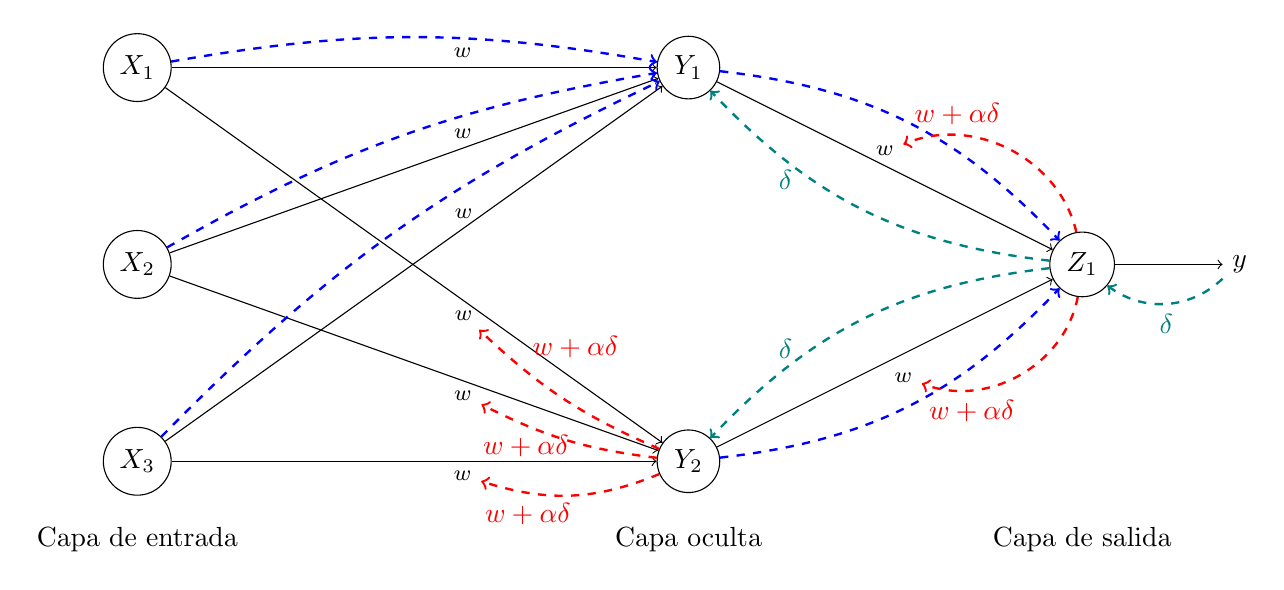
\begin{tikzpicture}

	\tikzstyle{nodo}=[circle, draw, minimum size=5ex]
	\tikzstyle{upw}=[dashed, red, ->, line width = 1pt]
	\tikzstyle{bold}=[line width=0.2ex]

	\coordinate (l_0) at (0, 3.5);
	\coordinate (l_1) at (7, 3.5);
	\coordinate (l_2) at (14, 3.5);
	\coordinate (input) at (0, -3.5);
	\coordinate (hidden) at (7, -3.5);
	\coordinate (output) at (12, -3.5);

	\coordinate (f_1_1) at (0, 2.5); % CAPA ENTRADA
	\coordinate (f_1_2) at (0, 0); % CAPA ENTRADA
	\coordinate (f_1_3) at (0, -2.50); % CAPA ENTRADA
	\coordinate (f_2_1) at (7, 2.5); % CAPA OCULTA 1
	\coordinate (f_2_2) at (7, -2.5); % CAPA OCULTA 1
	\coordinate (f_3_1) at (12, 0); % CAPA SALIDA
	\coordinate (f_out) at (14, 0); % CAPA SALIDA

	\node[] (input) at (input) {Capa de entrada};
	\node[] (hidden) at (hidden) {Capa oculta};
	\node[] (output) at (output) {Capa de salida};

	\node[nodo] (f_1_1) at (f_1_1) { $X_1$}; % CAPA ENTRADA
	\node[nodo] (f_1_2) at (f_1_2) { $X_2$}; % CAPA ENTRADA
	\node[nodo] (f_1_3) at (f_1_3) { $X_3$}; % CAPA ENTRADA
	\node[nodo] (f_2_1) at (f_2_1) { $Y_1$}; % CAPA OCULTA 1
	\node[nodo] (f_2_2) at (f_2_2) { $Y_2$}; % CAPA OCULTA 1
	\node[nodo] (f_3_1) at (f_3_1) { $Z_1$}; % CAPA SALIDA
	\node (f_out) at (f_out) {$y$}; % SALIDA


	\draw[->, font=\footnotesize] (f_1_1) --  node[pos=0.60, above] (w_1_1) {$w$} (f_2_1);
	\draw[->, font=\footnotesize] (f_1_2) --  node[pos=0.60, above] (w_1_2) {$w$} (f_2_1);
	\draw[->, font=\footnotesize] (f_1_3) -- node[pos=0.60, above] (w_1_3) {$w$} (f_2_1);
	\draw[->, font=\footnotesize] (f_1_1) -- node[pos=0.60, below] (w_2_1) {$w$} (f_2_2);
	\draw[->, font=\footnotesize] (f_1_2) -- node[pos=0.60, below] (w_2_2) {$w$} (f_2_2);
	\draw[->, font=\footnotesize] (f_1_3) -- node[pos=0.60, below] (w_2_3) {$w$} (f_2_2);

	\draw[->, font=\footnotesize] (f_2_1) -- node[midway, above ] (w_3_1) {$w$} (f_3_1);
	\draw[->, font=\footnotesize] (f_2_2) -- node[midway, below right] (w_3_2) {$w$} (f_3_1);

	\draw[->, font=\footnotesize] (f_3_1) -- (f_out);
	%%%%%%%%%%%%%%%%%%%%%%%%%%%%%%%%%
	%%%%%%%%%%%%%%%%%%%%%%%%%%%%%%%%%
	%%%%%%% PROPAGACIÓN DE LA SEÑAL %%%%%%%%
	\draw[upw, bold, blue] (f_1_1) to [bend left=10] (f_2_1);
	\draw[upw, bold, blue] (f_1_2) to [bend left=10] (f_2_1);
	\draw[upw, bold, blue] (f_1_3) to [bend left=10] (f_2_1);

	\draw[upw, bold, blue] (f_2_1) to [bend left=20] (f_3_1);
	\draw[upw, bold, blue] (f_2_2) to [bend right=20] (f_3_1);
	%%%%%%%%%%%%%%%%%%%%%%%%%%%%%%%%%
	%%%%%%%%%%%%%%%%%%%%%%%%%%%%%%%%%

	%%%%%%%%%%%%%%%%%%%%%%%%%%%%%%%%%
	%%%%%%%%%%%%%%%%%%%%%%%%%%%%%%%%%
	%%%%%%%% PROPAGACIÓN DEL ERROR %%%%%%%%
	\draw[upw, bold, teal] (f_out) to [bend left=40] node[below] {$\delta$} (f_3_1);
	\draw[upw, bold, teal] (f_3_1) to [bend left=20] node[near end, below] {$\delta$} (f_2_1);
	\draw[upw, bold, teal] (f_3_1) to [bend right=20] node[near end, above] {$\delta$} (f_2_2);
	%%%%%%%%%%%%%%%%%%%%%%%%%%%%%%%%%
	%%%%%%%%%%%%%%%%%%%%%%%%%%%%%%%%%


	%%%%%%%%%%%%%%%%%%%%%%%%%%%%%%%%%
	%%%%%%%%%%%%%%%%%%%%%%%%%%%%%%%%%
	%%%%%%% ACTUALIZACIÓN DE PESOS %%%%%%%%
	\draw[upw, bold] (f_3_1) to [bend right=50] node[above, near end] {$w + \alpha \delta$} (w_3_1);
	\draw[upw, bold] (f_3_1) to [bend left=50] node[below, near end] {$w + \alpha \delta$} (w_3_2);

	\draw[upw, bold] (f_2_2) to [bend left=10] node[above right, near end] {$w + \alpha \delta$} (w_2_1);
	\draw[upw, bold] (f_2_2) to [bend left=10] node[below, near end] {$w + \alpha \delta$} (w_2_2);
	\draw[upw, bold] (f_2_2) to [bend left=20] node[below, near end] {$w + \alpha \delta$} (w_2_3);
	%%%%%%%%%%%%%%%%%%%%%%%%%%%%%%%%%
	%%%%%%%%%%%%%%%%%%%%%%%%%%%%%%%%%
\end{tikzpicture}
